% ************ Chapter 3 ************
\chapter{Requisitos} 
\label{cap:3}
%Pretendia-se que fosse desenvolvido um sistema de informação completo para armazenar os registos feitos na fábrica. 

\section{Primeiro levantamento de requisitos}
Antes de iniciar qualquer tipo de desenvolvimento ou implementação, era fulcral definir uma lista de requisitos, que descreve-se de uma forma muito exata e clara o que se esperava que a solução implementada fosse. Logo na primeira reunião foi entregue um primeira lista de requisitos. Esta lista foi dividida em dois tipos diferentes: os primeiros são designados por Requisitos Absoluto e são requisitos com um grande nível de detalhe sobre as suas características e perspetivas. Os segundos são designados por Requisitos Indexados e são requisitos sobre os quais não se tem certeza sobre a totalidade das suas características ou dependem da informações externas. Os requisitos pertencentes a este último grupo devem passar por um processo de definição de modo a que se tornem requisitos absolutos.
Na primeira reunião com a administração foi entregue uma primeira lista de requisitos.\\
\\
Requisitos absolutos:
\begin{itemize}
	\item A aplicação só poderia ser acessível da rede interna
	\item Uso de uma base de dados relacional
	\item Registo do horário de entrada e saída dos colaboradores
	\item Registo do peso e ponto de recolha de onde vinha a matéria prima
	\item Registo do peso de cera, metal e plástico de uma produção, bem como o colaborador associado.
	\item Registo do peso do produto final acabado
	\item Registo da saída de produto acabado e cliente a quem foi vendido
	\item Impressão de uma segunda via dos códigos de barras já impressos referente a uma recolha ou um produto acabado
	\item Incremento do peso de uma recolha efetuada anteriormente.
	\item Zona protegida por ID e Password para a consulta dos registos feitos
	\item Possibilidade de editar e apagar registos já feitos.
	\item Script de analise da coerência dos dados registados.
\end{itemize}
Requisitos indexados:
\begin{itemize}
	\item Melhoria do design da base de dados
	\item A aplicação deveria ser acessível em dispositivos moveis e computadores
	\item Incremento do peso de uma recolha
\end{itemize}
Terminada esta reunião foi iniciado um processo de estudo do sistema atualmente implementado, o funcionamento da fábrica de forma a desindexar os requisitos indexados e determinar novos requisitos por forma a ter a melhor descrição possível do sistema a ser implementado.

\section{Estudo do sistema existente}
O sistema existente na empresa, conforme descrito anteriormente, foi construído com recurso ao Microsoft Access. Era compostos por 5 ecrãs destintos utilizados para recolher a informação gerada na fábrica. Um dos aspetos que são evidentes desde inicio é a não coesão visual dos elementos.

\begin{figure}[h!]
	\centering
	
	\begin{subfigure}[c]{0.3\linewidth}
		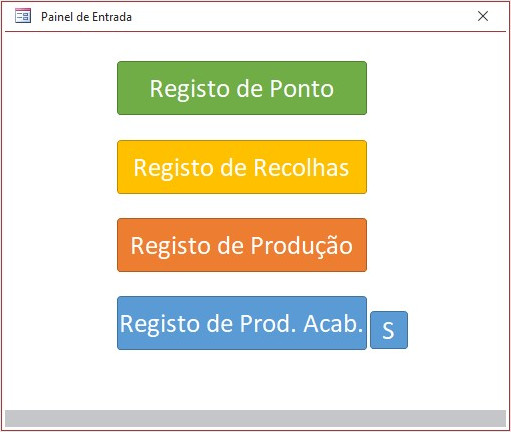
\includegraphics[width=\linewidth]{figuras/AppAccess/0-MenuInicial.jpg}
		\caption{Menu incial}
	\end{subfigure}
	\begin{subfigure}[c]{0.3\linewidth}
		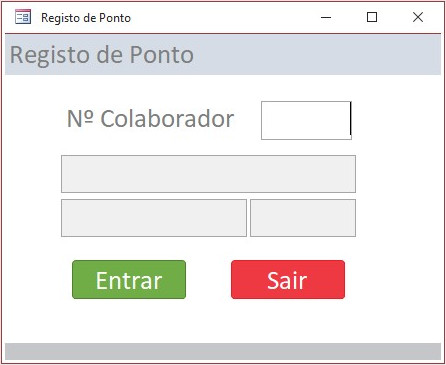
\includegraphics[width=\linewidth]{figuras/AppAccess/1-Ponto.jpg}
		\caption{Ecrã de marcação do ponto}
	\end{subfigure}
	\begin{subfigure}[c]{0.3\linewidth}
		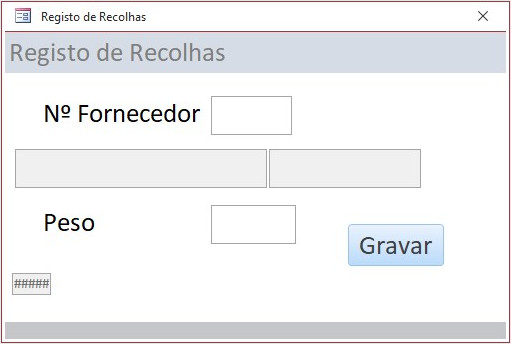
\includegraphics[width=\linewidth]{figuras/AppAccess/2-Recolha.jpg}
		\caption{Ecrã do registo de recolha}
	\end{subfigure}
	\begin{subfigure}[c]{0.3\linewidth}
		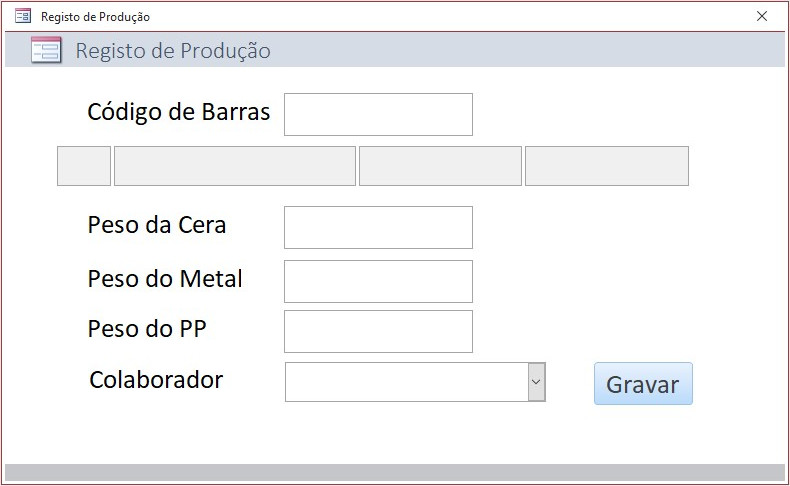
\includegraphics[width=\linewidth]{figuras/AppAccess/3-Producao.jpg}
		\caption{Ecrã do registo de produção}
	\end{subfigure}
	\begin{subfigure}[c]{0.3\linewidth}
		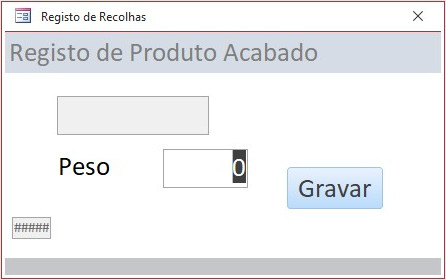
\includegraphics[width=\linewidth]{figuras/AppAccess/4-ProdutoAcabado.jpg}
		\caption{Ecrã do registo de produto acabado}
	\end{subfigure}
	\begin{subfigure}[c]{0.3\linewidth}
		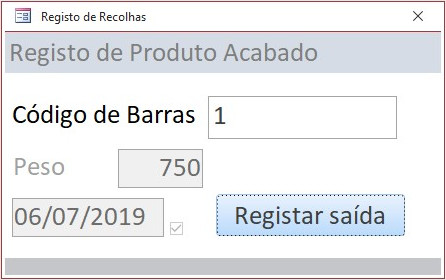
\includegraphics[width=\linewidth]{figuras/AppAccess/5-SaidaProdutoAcabado.jpg}
		\caption{Ecrã do registo de saída de produto acabado}
	\end{subfigure}
	
	\caption{Ecrãs da aplicação existe na empresa.}
	\label{fig:app_access}
\end{figure}

O fluxo dentro deste sistema era bastante simples também. Ao executar o ficheiro Microsoft Access, era apresentado diretamente o menu ao utilizador. Este selecionaria a opção referente ao registo que pretendia fazer e era apresentada numa nova janela o formulário correspondente. O utilizador preenchia com os dados requeridos e pressionava o botão "Gravar". Em caso de sucesso não era apresentado nenhuma mensagem. Em caso de erro era apresentada uma mensagem de a informar do erro. Esta mensagem era gerada diretamente pelo sistema de gestão de base de dados e não eram intuitivas. No caso de ser o registo de recolha ou de produto acabado, era ainda apresentado, numa nova janela um código de barras que seria impresso para identificar on elemento registado (figura \ref{fig:app_access_cb}). Estes códigos de barras deveriam ter estruturas diferentes. O código de barras referente à recolha (figura \ref{fig:app_access_cb} a) deveria ser constituído pelo código de barras correspondente ao ID, o ID do ponto de recolha e a data da recolha. Já no produto acabado era apenas apresentado o código de barras referente ao ID (figura \ref{fig:app_access_cb} b). A pedido da administração deveria passar a ser apresentado o código de barras em formato numérico no caso do produto acabado.

\begin{figure}[H]
	\centering
	
	\begin{subfigure}[t]{0.4\linewidth}
		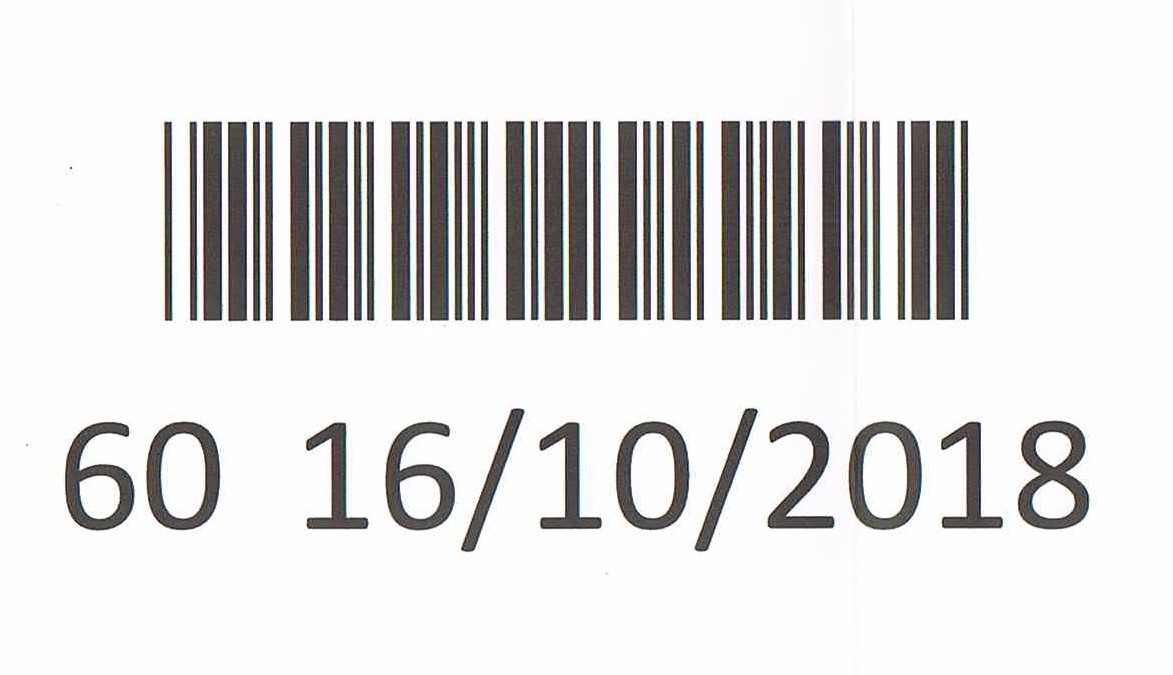
\includegraphics[width=\linewidth]{figuras/AppAccess/2-CodBarras.jpg}
		\label{fig:app_access_cb_recolha}
		\caption{Recolha}
	\end{subfigure}
	\begin{subfigure}[t]{0.4\linewidth}
		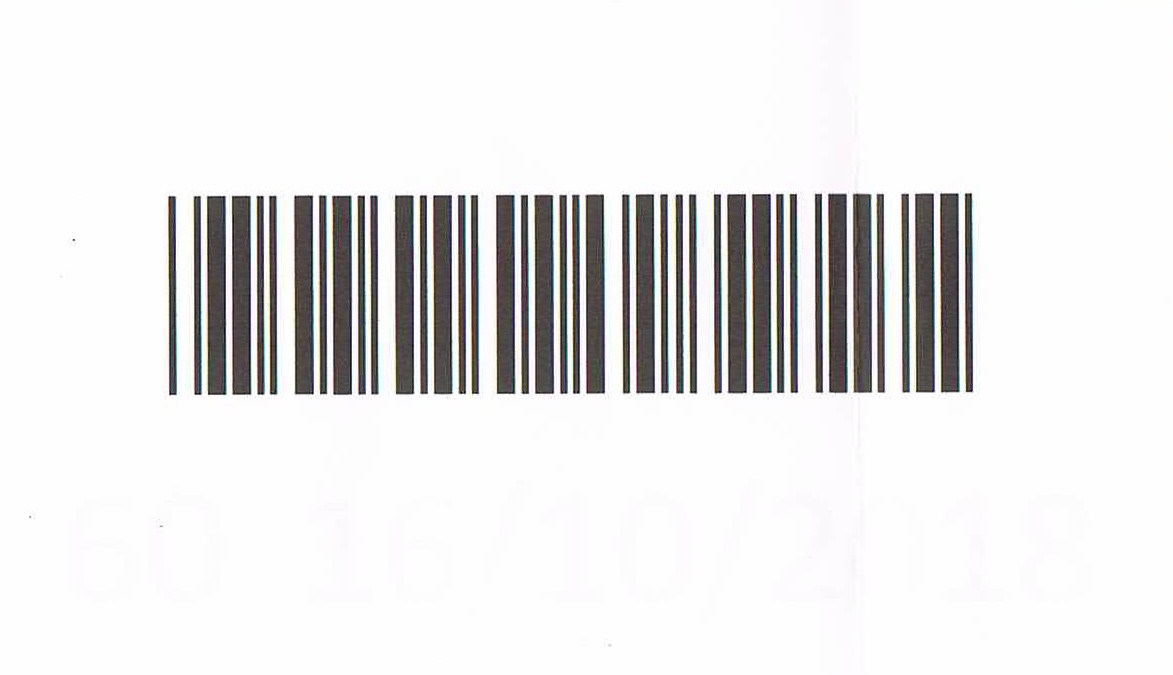
\includegraphics[width=\linewidth]{figuras/AppAccess/5-CodBarras.jpg}
		\label{fig:app_access_cb_prod_acabado}
		\caption{Produto Acabado}
	\end{subfigure}
	
	\caption{Exemplo dos códigos de barras gerados}
	\label{fig:app_access_cb}
\end{figure}


Após o estudo da aplicação foi iniciado o estudo da base de dados. Este estudo consistiu em compreender as tabelas que constituem base de dados, as suas relações e a informação que nelas é registada. Foi solicitado pela empresa sugestões de melhoria do design da base de dados com foco na coerência da informação registada.

\section{Modo de implementação do projeto}
Numa das reuniões discutiu-se o modo como o novo sistema deveria ser implementado. No dia em que ocorresse a primeira implementação do novo sistema, este deveria substituir por completo a aplicação construída no Microsoft Access. Isto porque devido à natureza da informação registada e tendo em conta que a base de dados teria a sua estrutura modificada, não era possível existir um período hibrido onde as duas aplicações coexistiram. Assim ficou definido que enquanto o novo sistema não fosse capaz de registar o ponto dos colaboradores, as recolhas efetuadas, as produções feitas, o produto finalizado e a sua saída, a implementação não iria ocorrer. Devido a este motivo um novo requisito foi criado: A aplicação deveria passar por um rigoroso conjunto de testes, que evolvessem não so a validação da informação registada como da experiencia de utilização de forma a minimizar ao máximo situações de erro que obrigassem a empresa a parar a sua atividade para corrigir a falha. Este testes deveriam ser independentes dos testes feitos no desenvolvimento e seriam feitos pelos elementos da administração e numa fase posterior, por alguns colaboradores de empresa num ambiente de teste.

\section{Último levantamento de requisito}
Todos os requisitos da aplicação ficaram definidos no final da primeira semana, à excepção dos requisitos referentes a uma funcionalidade de nova que a administração pretendia implementar, o incremento do peso de uma recolha. Em algumas recolhas efetuada, o peso total da recolha superava a capacidade de ser pesado de uma so vez, seja pelo peso de matéria prima seja pela quantidade. Apesar de estar consciente desta necessidade a administração sugeriu deixar a discussão sobre esta nova funcionalidade para o pós primeira implementação. Não se tratava de uma funcionalidade fundamental para o sistema e como tal havia a intenção de estudar a melhor forma de implementar esta solução. Solução essa que foi discutida na sétima semana do período de estágio. Consistiu na criação de uma nova tabela "Completar Recolha" que iria armazenar o histórico de incrementos feitos numa recolha, para assim poder identificar eventuais erros no registos da informação. Do ponto de vista da aplicação a recolha a ser incrementada seria identificada pelo código de barras impresso anteriormente e deveria ser apresentado ao utilizador o histórico de incrementos referente a essa recolha. Por fim definiu-se que uma recolha registada com o peso de zero quilos deveria redirecionar automaticamente o utilizador para o ecrã do incremento desta recolha após a impressão do primeiro código de barras.

\section{Lista final de requisitos}
Após as todas as reuniões de levantamento de requisitos, chegou-se à seguinte lista composta apenas por requisitos absolutos.
\begin{itemize}
	\item A aplicação só poderia ser acessível da rede interna
	\item Aplicação alojada num servidor físico com Ubuntu Server 18.04
	\item Aplicação WEB desenvolvida em PHP, com o framework Laravel, e em Javascrip.
	\item A aplicação teria de seguir o modelo MVC\label{sym:MVC}
	\item A aplicação deve ser construída de forma modular de forma a facilitar a sua manutenção no futuro
	\item Uso de uma base de dados relacional, construida com o sistema de gestão de base de dados Microsoft SQL Server e a estrutura aprovada pela administração.
	\item A implementação teria de ser feita em duas fases, uma primeira onde se substituía totalmente a aplicação existente na fabrica (Registo de ponto, de recolhas, de produção, de produto acabado e de saída de produto acabado), de modo a não parar o trabalho da fábrica ou ter de usar duas aplicações e uma segunda fase durante a qual as novas funcionalidades seriam aplicadas incrementalmente
	\item Devido à utilização de uma base de dados completamente reestruturada, antes da primeira implementação a aplicação teria de passar por uma fase de testes muito exigente para impedir erros que obrigassem ao uso da base de dados antiga.
	\item Os teste que irão aprovar a passagem do novo sistema ao estado de produção deverão ser independestes do testes de desenvolvimento e serão feitos, numa primeira fase pela administração. Quando atingirem um nível de maturidade que satisfaz as expectativas da administração a aplicação deverá ser testada, num ambiente de testes, por alguns colaboradores da empresa.
	\item O sistema tem de ser graficamente coeso
	\item O novo sistema terá de ter um impacto minimo no modo de utilização dos funcionários.
	\item Mensagens do sistema após cada ação
	\item Mensagens com linguagem simples e direta
	\item Registo do horário de entrada e saída dos colaboradores
	\item Registo do peso e ponto de recolha de onde vinha a matéria prima
	\item Possibilidade de incrementar o peso de uma recolha
	\item Se a recolha fosse iniciada com 0kg (zero quilogramas) é iniciado automaticamente o processo de incremento do peso da recolha que acabou de ser registada.
	\item Impressão de um código de barras com o ID gerado para a recolha inserida, id do ponto de recolha e data de recolha
	\item Registo do peso de cera, metal e plástico de uma produção, bem como o colaborador associado.
	\item Registo do peso do produto final acabado
	\item Impressão de um código de barras com o ID gerado para a produto final acabado
	\item Registo da saída de produto acabado e cliente a quem foi vendido
	\item Impressão de uma segunda via dos códigos de barras já impressos referente a uma recolha ou um produto acabado
	\item Incremento do peso de uma recolha efetuada anteriormente.
	\item Após o incremento do peso deveria ser impresso uma segunda via do código de barras dessa mesma recolha.
	\item Zona protegida por ID e Password para a consulta dos registos feitos
	\item As tabelas apresentadas na interface da aplicação teriam de ser capazes de refletir alterações na estrutura das tabelas da base de dados.
	\item Possibilidade de registar e apagar utilizadores na plataforma.
	\item Possibilidade de registar e apagar colaboradores.
	\item Possibilidade de registar e apagar Pontos de Recolha.
	\item Possibilidade de registar e apagar Clientes.
	\item Possibilidade de editar e apagar registos já feitos.
	\item Possibilidade de inserir/editar/apagar/executar comandos SQL personalizados.
	\item Script de analise da coerência dos dados registados para Pontos de Recolha, Registos de Ponto e Produção.
\end{itemize}